\section{Experiments}
\label{sec:experiments}

%We have argued the case for using measurements of the latent moments to 
%aid parameter estimation.
The spectral decomposition (Steps 1 and 2) in \sectionref{measurements}
provides estimates of the latent moments,
which are used in the optimization problem \equationref{minKL}.
In this section, we study our approach empirically.
%seek to answer two questions empirically:
%(i) how much do the measurements aid estimation, and
%(ii) how effectively are the measurements estimated using the
%method of moments.
%We found that measurements can improve the fit of the
%parameters estimated considerably.
%While empirical measurements estimated using the
%method of moments are less accurate, we still find that they improve
%parameter estimates in general.

% Could it be effective in practice?
\paragraph{General results}

For both the mixture model and HMM,
we generated 5 different models and $n=10,000$ examples from the model.
\tableref{errors} shows the prediction accuracy averaged over the 5 models and 5
random trials each.
We see that using latent moments recovered from spectral decomposition
helps over EM, especially for the mixture model.

\paragraph{Effect of latent moments}

We generated 10 random HMMs,
each with $k=3$ hidden states and $\ell=5$ possible observed values. 
For each model, we generated $n=10,000$ sequences of length $L=3$.
We compared the prediction error (averaged over 10 trials) using EM
initialized using \equationref{minKL} when different percentages of the expected
latent moments were observed.

%For example, we ran one experiment where we assumed 10\% of the latent
%measurements were observed.

%\begin{figure}
%  \centering
%  \begin{subfigure}[b]{0.4\textwidth}
%    \begin{tabular}{l | l l }
%        Algorithm / $(k,\ell)$ & $(3,3)$ & $(3,5)$ \\ \hline
%        & \multicolumn{2}{c}{Mixture model} \\
%        EM                    & 0.51 & 0.72 \\
%        Spectral              & 0.68 & 0.80 \\
%        Oracle                & 0.70 & 0.80 \\ \hline
%        & \multicolumn{2}{c}{HMM} \\
%        EM                    & 0.42 & 0.62  \\
%        Spectral              & 0.45 & 0.64  \\
%        Oracle                & 0.47 & 0.73
%    \end{tabular}
%    \caption{Micro-averaged accuracy.}
%    \label{tab:errors}
%  \end{subfigure}
%  \begin{subfigure}[b]{0.4\textwidth}
%    %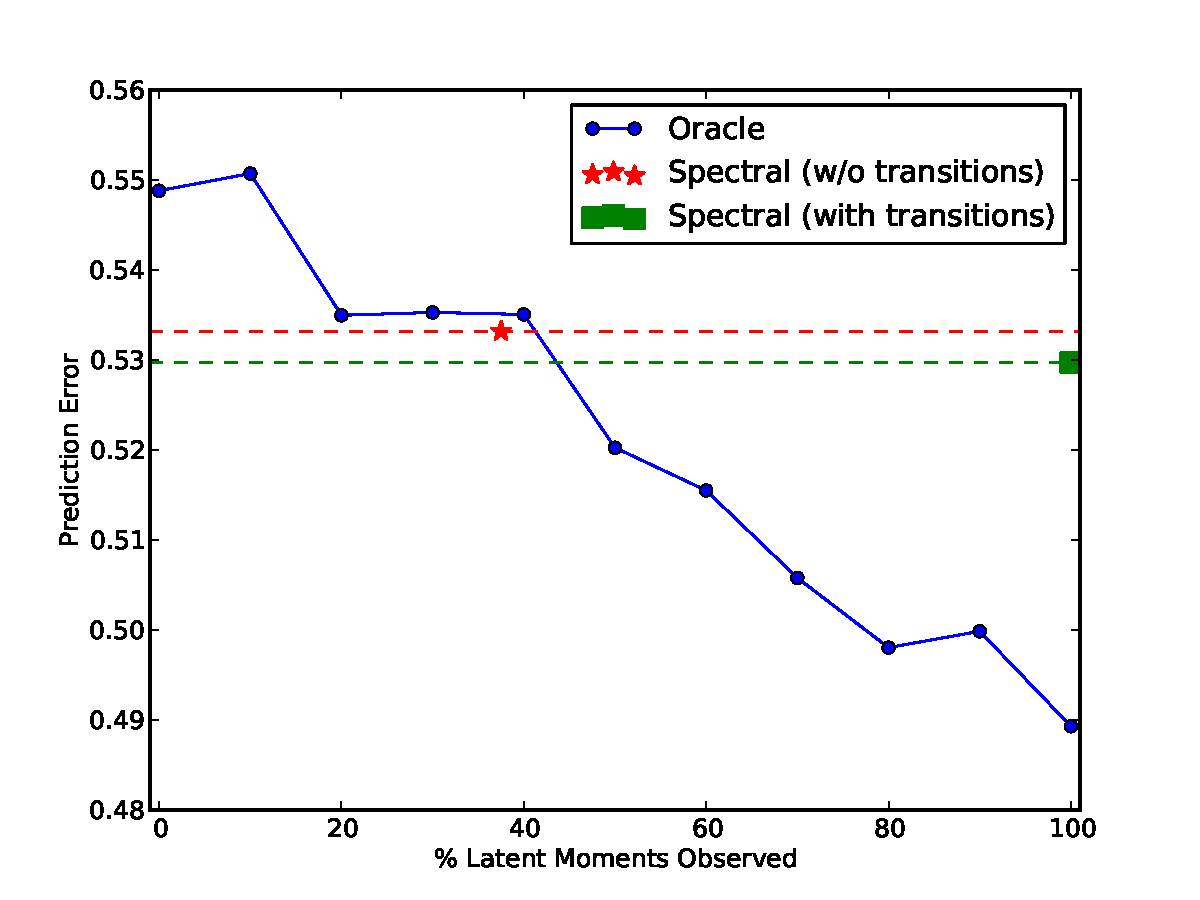
\includegraphics[width=1.0\textwidth]{figures/measurements.pdf}
%    \caption{Prediction accuracy.}
%    \label{fig:measurements}
%  \end{subfigure}
%  \caption{Experimental results.  Spectral: using latent moments estimated from
%  spectral decomposition.  Oracle: using expected moments under the true
%  parameters.}
%\end{figure}

%\Fig{figures/measurements}{0.3}{measurements}{Prediction Accuracy}

\figureref{measurements}
shows the prediction error of the parameters
micro-averaged over the different data and models.  First, as we use
more expected latent moments (oracle), prediction error decreases.  Second,
learning from only the emissions moments is comparable
to using emissions and transitions, verifying the fact that
we can effectively leverage from partial information.\footnote{
These errors are high relative to the oracle due to sampling error.}

%For comparison, we have
%included the accuracy achieved using the method of moments estimation procedure
%described in \refsec{factorization} with empirical moment estimates.  We see
%that using measurements for even a small percentage of features can improve
%prediction accuracy by \todo{x\%}. Spectral estimates too improve accuracy,
%though not as markedly; we observed a \todo{x\%} improvement.

% - we ran experiments with different proportions of the expected feature counts being observed and plot performance here. 
% - while such information is not available in practice, we note that it provides a significant improvement over learning with just EM.
% - next, we used spectral techniques to estimate the counts on the data and observed that it also showed a concrete improvement in performance, though not as much as the measurements.

% details:
% - For purposes of illustration, we looked at 10 different hmms with
% parameters $K=3$, $D=5$ and $N=10^5$ samples. We ran each experiment for
% 10 different data samples and report the micro-averages.

%\begin{table}
%    \label{tab:errors}
%    \begin{tabular}{l | l l | l l l }
%        Algorithm & $k$ & $d$ & Accuracy & $\Delta \hat \E[\phi(x,h)]$ & Log Likelihood \\ \hline
%        & \multicolumn{2}{|c|}{Mixtures} & & & \\ \hline
%        \multirow{3}{*}{EM} 
%        & 3 & 2 & 0.65 (+/- 0.01) & 1.23 & -3.72 \\
%        & 3 & 3 & 0.51 (+/- 0.06) & 1.81 & -4.21\\
%        & 5 & 2 & 0.72 (+/- 0.07) & 1.13 & -5.21\\ \hline
%        \multirow{3}{*}{Spectral} 
%        & 3 & 2 & 0.80 (+/- 0.09) & 0.23 & -3.54 \\
%        & 3 & 3 & 0.68 (+/- 0.10) & 1.01 & -3.76 \\
%        & 5 & 2 & 0.80 (+/- 0.05) & 0.18 & -5.04 \\ \hline
%        \multirow{3}{*}{100\% Measurements} 
%        & 3 & 2 & 0.80 (+/- 0.08) & 0.01& -3.54 \\
%        & 3 & 3 & 0.70 (+/- 0.11) & 0.02& -3.87 \\
%        & 5 & 2 & 0.80 (+/- 0.05) & 0.01& -5.03 \\ \hline
%        & \multicolumn{2}{|c|}{HMMs} & & & \\ \hline
%        \multirow{3}{*}{EM} 
%& 3 & 2 & 0.64 (+/- 0.10) & 1.71 & -4.51 \\  
%& 3 & 3 & 0.42 (+/- 0.05) & 2.41 & -6.09 \\  
%& 5 & 2 & 0.62 (+/- 0.09) & 1.60 & -6.47 \\  \hline
%        \multirow{3}{*}{Spectral} 
%& 3 & 2 & 0.67 (+/- 0.07) & 2.59 & -3.71 \\ 
%& 3 & 3 & 0.45 (+/- 0.08) & 4.96 & -4.36 \\ 
%& 5 & 2 & 0.64 (+/- 0.10) & 3.43 & -5.31 \\ \hline
%        \multirow{3}{*}{100\% Measurements} 
%& 3 & 2 & 0.71 (+/- 0.07) & 0.39 & -4.64 \\ 
%& 3 & 3 & 0.47 (+/- 0.07) & 1.53 & -5.85 \\ 
%& 5 & 2 & 0.73 (+/- 0.07) & 0.39 & -6.16 \\ \hline
%    \end{tabular}
%    \caption{Micro-averaged Errors.}
%\end{table}

%In the table, we compare randomly initialized EM with EM initialized using (a)
%empirical measurements estimated with the method of moments and (b) fully
%expected measurements.

%First, we note that we found measurements to uniformly improve the prediction
%accuracy of EM. The picture for method of moments is similar, though there is
%greater variation in the improvement it provides.

% - Generated data from different 3-view mixture models and hmms. 
% - Each averages over 5 different parameters and 5 different data samples.
% - Find that there is quite some variation in spectral performance, but measurements uniformly helps estimation.

% \subsection{Basic mixture model}
% 
% Show simple mixture model works on artifical data.
% 
% Show EM/gradient gets stuck in local optima.
% 
% spectral methods are not statistically efficient (especially with parameter sharing).
% 
% \subsection{Measurements}
% 
% For models in \reffig{generalModels}, do experiments.
% 
% Show that the non-convexity decreases.
% 
% \subsection{Factorial models}
% 
% Show that the unshuffling basically works with near infinite data, while EM gets stuck in local optima.
% 
% \subsection{Part-of-speech induction}
% 
% \cite{kirkpatrick10painless} trains for 1,000 iterations, which takes a long time.
% 63.1\% Basic HMM
% 68.1\% EM, L-BFGS 75.5\%
% 
% Can we match the performance?
% 
% Also, since method of moments doesn't require inference, can we use a much larger corpus
% and get better results.


